\chapter{Syntax-Translation Mechanism}

In this chapter, we will define our syntax-translation function which maps Haskell expression to Prolog expression. In order to do that, I will introduce you a first approach to it and then, we will see so many examples of what kind of changes it does and how to do that.\\\\
%%
First of all, we will see a basic scenario where algebra data types are defined with fixed types, i.e., the monomorphic type cases. We will see how to translate primitive types and I will provide so many functions that help us to get those primitive types values guided by the syntax of Haskell's types. That is, what we need to translate the syntax of the type expression \ttt{Int}, \ttt{String}, or \ttt{Bool} is usually used in the Haskell functions or ADTs declaration to a Prolog program. Then, we will see what is the equivalent expression for some trivial algebra data types like \textit{Maybe}, \textit{Either}, \textit{Binary Tree}, and so on.\\\\
%%
We will talk about what kind of problems those generations carry on and how to deal with them. And finally, we will talk about polymorphism and the way for generating a value related to the equivalent Prolog \textit{type} for a given Haskell's algebra data type declaration with polymorphic types. The purpose is to generalize those changes based on the translation of Haskell's formal grammar step by step doing refinements from the step back to the next one in a progressive improvement process.

\section{Monomorphic Types} \label{ch:monomorphic-types}

For our first steps, we can deal with the most basic case: those scenarios where ADT expressions are defined with monomorphic types. To do that, we can avoid keeping in mind the type or fixing the type expression in the formal grammar definition and simply try to generate their structure with it.\\
%%

Let's define the syntax translation function. Let $\mathcal{H}$, $\mathcal{P}$ be the set of well-defined expressions in Haskell and Prolog, respectively. We can consider $\mathcal{H}_{\ttt{ADT}}$ and $\mathcal{P}_{\text{Clause}}$, the subset of well-defined algebra data types expressions in Haskell contained in $\mathcal{H}$ and the subset of clauses in $\mathcal{P}$, respectively. Following the formal grammar definition for algebra data type expressions in Haskell:
\begin{align*}
	\ttt{data} \tav simpletype =  & \tav constrs                                                                       &   &   \\
	                              & \updownsquigarrow                                                                  &   &   \\
	\ttt{data} \tav tycon \tav 	= & \tav constr_1 \tav | \tav constr_2 \tav | \tav \ldots \tav | \tav constr_n         &   &   \\
	                              & \updownsquigarrow                                                                  &   &   \\
	\ttt{data} \tav tycon \tav 	= & \tav con_1 \tav atype_{1,1} \tav atype_{1,2} \tav \ldots \tav atype_{1,k_1} \tav | &   &   \\
	                              & \tav con_2 \tav atype_{2,1} \tav atype_{2,2} \tav \ldots \tav atype_{2,k_2} \tav | &   &   \\
	                              & \tav \vdots \tav                                                                   &   &   \\
	                              & \tav con_n \tav atype_{n,1} \tav atype_{n,2} \tav \ldots \tav atype_{n,k_n} \tav | &   &   \\
\end{align*}
We define our syntax-tranlsation semantic $$\text{HSyntax} :\tav \mathcal{H}_{\ttt{ADT}} \tav \longrightarrow \tav \mathcal{P}_{\text{Clause}}$$ for monomorphic types as is shown in appendix ~\ref{subsec:monomorphic-types-function}.\\\\
%%
Now we have defined our syntax-translation semantic for monomorphic types, we will see some examples that help us to understand better. But before that, I will introduce you generation functions for primitive types.
%%
\subsection{Primitive Types generators}
For this work, I provide some kind of Prolog programs that will be useful to us to generate primitive types. These implementations are not the best efficient ones, but they are enough for our purpose. We need those generators in the case when $tycon$ is a primitive type, because $$\sem{GSyntax}{tycon} = gen\_\sem{Lower}{tycon}$$
%%
\subsubsection{\ttt{Char} type generator}
\lstinputlisting[language=Prolog, label=char-type-generator]{sections/code/chapter3/types/char.pl}
%%
\subsubsection{\ttt{String} type generator}
There is a predicate \ttt{string} in the Prolog's prelude to check if an expression is a string or not. Therefore, we will provide just the \ttt{gen\_string} rule.
\lstinputlisting[language=Prolog, label=string-type-generator]{sections/code/chapter3/types/string.pl}
%%
\subsubsection{\ttt{Int} type generator}
\lstinputlisting[language=Prolog, label=int-type-generator]{sections/code/chapter3/types/int.pl}
%%
\subsubsection{\ttt{Integer} type generator}
There is a predicate \ttt{string} in the Prolog's prelude to check if an expression is a string or not. Therefore, we will provide just the \ttt{gen\_string} rule. For our purpose, we don't need all the integer type sets, so here we decided to bound for a good enough range.
\lstinputlisting[language=Prolog, label=integer-type-generator]{sections/code/chapter3/types/integer.pl}
%%
\subsubsection{\ttt{Bool} type generator}
\lstinputlisting[language=Prolog, label=bool-type-generator]{sections/code/chapter3/types/bool.pl}
%%
\subsubsection{\ttt{Unit} type generator}
\lstinputlisting[language=Prolog, label=unit-type-generator]{sections/code/chapter3/types/unit.pl}
%%
\subsubsection{\ttt{Double} type generator}
In Prolog, \ttt{float} predicate is a \textit{representation type}. You can have a numeric value that has a representation both as integer and float and these representations are distinguishable: values $1 \equiv 1.0$ but expressions $\ttt{1} \neq \ttt{1.0}$.
\lstinputlisting[language=Prolog, label=double-type-generator]{sections/code/chapter3/types/double.pl}
%%
\subsection{Examples} \label{ch:monomorphic-types-examples}
%%
%%
\begin{example}[MaybeInt]
	Let's suppose the following Haskell ADT definition:
	\lstinputlisting[language=Haskell, label=maybeint-haskell-monotype]{sections/code/chapter3/monotypes/haskell/maybeint-monotype.hs}
	Here, using the translation function defined above as is shown in appendix ~\ref{subsec:monomorphic-types-translation-maybeint}, we can translate the Haskell definition shown above to the following Prolog program:\\
	\lstinputlisting[language=Prolog, label=maybeint-prolog-monotype]{sections/code/chapter3/monotypes/prolog/maybeint-monotype.pl}
	Now, if you type \ttt{maybeint(X)} in the Prolog's CLI, you will get a valid \ttt{MaybeInt} generated value.
\end{example}
%%
%%
\begin{example}[Non-Polymorphic Either]
	Let's suppose our non-polymorphic version of the definition of Either in Haskell for both \ttt{String} and \ttt{Int} types:
	\lstinputlisting[language=Haskell, label=either-haskell-monotype]{sections/code/chapter3/monotypes/haskell/either-monotype.hs}
	Here, using the translation function defined above as is shown in appendix ~\ref{subsec:monomorphic-types-translation-either}, we can translate the Haskell definition shown above to the following Prolog program:\\
	%%
	\lstinputlisting[language=Prolog, label=either-prolog-monotype]{sections/code/chapter3/monotypes/prolog/either-monotype.pl}
	%%
	Now, if you type \ttt{either(X)} in the Prolog's CLI, you will get a valid \ttt{Either} generated value.
\end{example}
%%
%%
\begin{example}[MyListBool]
	Let's suppose the following Haskell ADT definition:
	\lstinputlisting[language=Haskell, label=mylistbool-haskell-monotype]{sections/code/chapter3/monotypes/haskell/mylistbool-monotype.hs}
	%%
	We can observe it is a recursive definition, so the question is, what happens with the declaration of $\ttt{MyListBool}$ in its own declaration. Well, as \ttt{MyListBool} is a Haskell algebra data type, we can deal with it as we have been doing in a recursively way or, in another hand, we can define the Prolog rule as a recursive rule (explained in section ~\ref{ch:recursive-rules}).\\\\
	%%
	Therefore, using the translation function defined above as is shown in appendix ~\ref{subsec:monomorphic-types-translation-mylistbool}, we can translate the Haskell definition shown above to the following Prolog program:\\
	%%
	\lstinputlisting[language=Prolog, label=mylistbool-prolog-monotype]{sections/code/chapter3/monotypes/prolog/mylistbool-monotype.pl}
	%%
	Now, if you type \ttt{mylistbool(X)} in the Prolog's CLI, you will get a valid \ttt{MyListBool} generated value. But, what happens here? Let's take a look at a few more examples before.
\end{example}
%%
%%
\begin{example}[Binary Search Tree]
	Here we go again... Let's suppose the following Haskell ADT definition:
	\lstinputlisting[language=Haskell, label=bst-haskell-monotype]{sections/code/chapter3/monotypes/haskell/bst-monotype.hs}
	%%
	We can observe it is a recursive definition, so the question is, what happens with the declaration of $\ttt{BSTree}$ in its own declaration. Well, as \ttt{BSTree} is a Haskell algebra data type, we can deal with it as we have been doing in a recursively way or, in another hand, we can define the Prolog rule as a recursive rule (explained in section ~\ref{ch:recursive-rules}).\\\\
	%%
	Therefore, using the translation function defined above as is shown in appendix ~\ref{subsec:monomorphic-types-translation-bstree}, we can translate the Haskell definition shown above to the following Prolog program:\\
	%%
	\lstinputlisting[language=Prolog, label=bst-prolog-monotype]{sections/code/chapter3/monotypes/prolog/bst-monotype.pl}
	%%
	Now, if you type \ttt{bstree(X)} in the Prolog's CLI, you will get a valid \ttt{BSTree} generated value. Again, what happens here? Did you see?\\
\end{example}
%%
%%
\begin{example}[SomeWeird]
	Let's suppose the following (really weird) Haskell ADT definition:
	\lstinputlisting[language=Haskell, label=someweird-haskell-monotype]{sections/code/chapter3/monotypes/haskell/someweird-monotype.hs}
	%%
	We can observe it is a recursive definition, so the question is, what happens with the declaration of $\ttt{SomeWeird}$ in its own declaration. Well, as \ttt{SomeWeird} is a Haskell algebra data type, we can deal with it as we have been doing in a recursively way or, in another hand, we can define the Prolog rule as a recursive rule (explained in section ~\ref{ch:recursive-rules}).\\\\
	%%
	Therefore, using the translation function defined above as is shown in appendix ~\ref{subsec:monomorphic-types-translation-someweird}, we can translate the Haskell definition shown above to the following Prolog program:\\
	\lstinputlisting[language=Prolog, label=someweird-prolog-monotype]{sections/code/chapter3/monotypes/prolog/someweird-monotype.pl}
	%%
	Now, if you type \ttt{someweird(X)} in the Prolog's CLI, you will get a valid \ttt{SomeWeird} generated value. Oh my god... it was so weird. Finally, let's take a look at one more example.\\
\end{example}
%%
%%
\begin{example}[Rose Tree]
	Last dance! Let's suppose the following Haskell ADT definition:
	\lstinputlisting[language=Haskell, label=rstree-haskell-monotype]{sections/code/chapter3/monotypes/haskell/rstree-monotype.hs}
	We can observe it is a recursive definition. Again, as \ttt{RSTree} is a Haskell algebra data type, we can deal with it as we have been doing in a recursively way or, in another hand, we can define the Prolog rule as a recursive rule (explained in section ~\ref{ch:recursive-rules}). Also, it is defined using Haskell's list type constructor which we have not yet discussed. \\
	%%
							
	Haskell lists are not really either an algebra data type or a primitive type. It is a kind of algebra structure which is not formally defined as a \ttt{data}-Haskell expression. Therefore, its implementation in Prolog is different. For now, we will implement a particular generator of lists of Rose Trees, but when we talk about polymorphism, I will provide a generic generator of lists of any type. So, here using the translation function defined above as is shown in appendix ~\ref{subsec:monomorphic-types-translation-rstree}, we can translate the Haskell definition shown above to the following Prolog program:\\
	%%
	\lstinputlisting[language=Prolog, label=rstree-prolog-monotype]{sections/code/chapter3/monotypes/prolog/rstree-monotype.pl}
	%%
	Now, if you type \ttt{rstree(X)} in the Prolog's CLI, you will get a valid \ttt{RSTree} generated value. Again, what happens here? Did you see it? No? Okay, let's talk.\\
\end{example}

\section{Monomorphic Types with Boundaries} \label{ch:monomorphic-types-boundaries}

When we try to generate recursively a structure in Prolog, it tries to get all the space that the symbolic variables hold for the rules that participate in the resolution process. Moreover, Prolog has default resolution strategies that imply directly in the returned solutions. We won't deep into those details, if you are interested in how to implement more efficient resolution strategies, you can check \cite{effgenttransf}. What we want to get is completeness, a good enough space of generated values for our purpose.\\\\
%%
To be more precise:
\begin{itemize}
	\item In the case of the \ttt{MyListBool} algebra data type, we are just getting those values with \ttt{true}. We never get either \ttt{Cons(false, Nil)} or \ttt{Cons(false, Cons(true, Cons(false, Nil)))}.
	\item In the case of \ttt{BSTree}, we are resolving deeply the right-branch side, getting always \ttt{nil} in the left-branch side, for example. Our Binary Search Tree Prolog program returns us: $$\ttt{T(-483997780, Nil, T(349868009, Nil, T(-265947283, Nil, Nil)))}$$ and never $$\ttt{T(-483997780, T(-265947283, Nil, Nil), T(349868009, Nil, Nil))}$$
	\item In the case of \ttt{RSTree}, we are resolving deeply the inner-list side instead of getting another Rose Tree value in the most out of the list. Our Rose Tree Prolog program returns us: $$\ttt{R(-193684758, [R(-178049475, [R(186461544, [])])])}$$ and never $$\ttt{R(-193684758, [R(-178049475, []), R(186461544, [])])}$$
\end{itemize}
%%
An approach that fits very well is to define boundaries for recursive structures. We can define the limit of elements in a list, or the depth in the branch of a binary search tree. For instance:\\\\
%%
Let's suppose the following Haskell ADT definition showed before:
\lstinputlisting[language=Haskell, label=mylistbool-haskell-monotype]{sections/code/chapter3/monotypes/haskell/mylistbool-monotype.hs}
We know that using the syntax-translate mechanism HSyntax defined in \ref{ch:monomorphic-types}, we obtaing the following Prolog program:
%%
\lstinputlisting[language=Prolog, label=mylistbool-prolog-monotype]{sections/code/chapter3/monotypes/prolog/mylistbool-monotype.pl}
%%
Let's consider a new variable \ttt{Length} that represents the length of \ttt{MyListBool}. We can refine our last program into this new one
\begin{lstlisting}[language=Prolog]
	mylistbool(0, nil).																								%% rule 1
	mylistbool(Length, cons(X21, X22)) :-															%% rule 2
		gen_bool(X21),
		Length > 0,
		N1 is Length - 1,
		mylistbool(N1, X22).			
\end{lstlisting}
For the base case when $\ttt{Length} = 0$, our program returns $Nil$. Otherwise, it returns  $$Cons(b_1, Cons(b2, ... Cons(b_n, Nil)))$$ Now, if you type \ttt{mylistbool(N, X)} in the Prolog's CLI, you will get a valid \ttt{MyListBool} generated value:
\begin{itemize}
	\item Let $\ttt{N} = 1$, our program returns:
	      \begin{eqnarray*}
	      	&&\ttt{cons(true, nil)}\\
	      	&&\ttt{cons(false, nil)}
	      \end{eqnarray*}
	\item Let $\ttt{N} = 2$, our program returns:
	      \begin{eqnarray*}
	      	&&\ttt{cons(true, cons(true, nil))}\\
	      	&&\ttt{cons(true, cons(false, nil))}\\
	      	&&\ttt{cons(false, cons(true, nil))}\\
	      	&&\ttt{cons(false, cons(false, nil))}
	      \end{eqnarray*}
\end{itemize}
We have just seen that just adding a variable allows us to get more control over the space of solutions. So, we need in some way to include this new feature in our syntax-translate mechanism as a refinement of the old one.\\\\
However, if we talk about the \ttt{MyListBool} algebra data type and how their expressions are constructed, we can define $\Gamma_{MyListBool}$ the set of expressions that define the structure of the elements belong to \ttt{MyListBool} type. $$\Gamma_{MyListBool} = \{ Nil, \tav Cons(b, Nil), \tav Cons(b, Cons(b, Nil)), \; \ldots \} \tav \tav b \in \ttt{Bool}$$
%%
And we can consider the binary operation $\preceq$ defined as, for all $e_1$, $e_2$ two expressions, we say that $e_1 \preceq e_2$ if the expression of $e_1$ is a subexpression contained in the expression $e_2$. Then, we can say that $(\Gamma_{MyListBool}, \preceq)$ is a poset, where $Nil$ is the minimal element.
\begin{align*}
	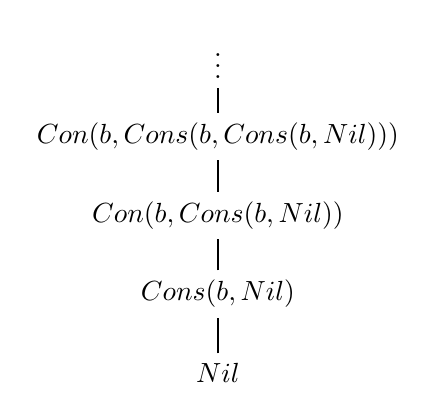
\begin{tikzpicture}                                   
	\node (a) at (0,3) {$\vdots$};                        
	\node (b) at (0,2) {$Con(b, Cons(b, Cons(b, Nil)))$}; 
	\node (c) at (0,1) {$Con(b, Cons(b, Nil))$};          
	\node (d) at (0,0) {$Cons(b, Nil)$};                  
	\node (min) at (0,-1) {$Nil$};                        
	\draw [thick](min) -- (d) -- (c) -- (b) -- (a);       
	\end{tikzpicture}                                     
\end{align*}
In this case, the structural induction of the \ttt{MyListBool} algebra data type grows in a linear-deep way. However, that \textit{easy} grow is not the only one.\\\\
%%
All right, let's take a look now at the \ttt{BSTree} expressions. In this case, we have a recursion definition in the two branches on the second constructor in the definition of \ttt{BSTree} algebra data type. The structural induction derives its shape in two possible nodes, the left one and the right one.\\\\
%%
Let $\Gamma_{BSTree}$ be the set of expressions that define the structure of an element in the \ttt{BSTree} type.
\begin{eqnarray*}
	\Gamma_{BSTree} & = & \{ Nil, \tav T(n, Nil, \; Nil), \\
	&& \tav T(n, \; T(n, Nil, \; Nil), \; Nil), \tav T(n, Nil, \; T(n, Nil, \; Nil)), \tav  \\
	&& \tav T(n, T(n, \; Nil, \; Nil), \; T(n, Nil, \; Nil)), \; \ldots \; \} \tav \tav n \in \ttt{Int}
\end{eqnarray*}
%%
Therefore, $(\Gamma_{BSTree}, \preceq)$ is a poset, where $Nil$ is the minimal element.
\begin{align*}
	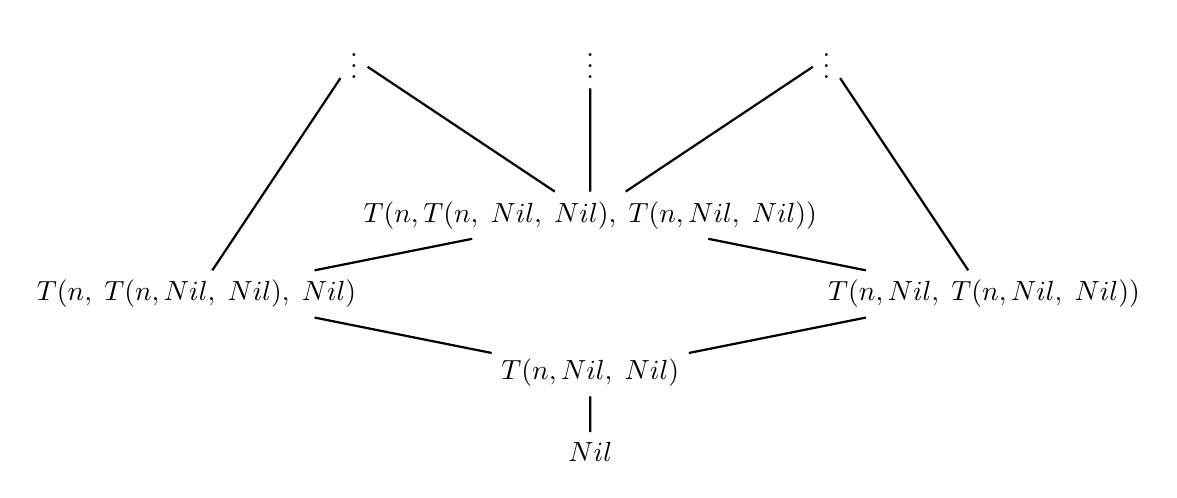
\begin{tikzpicture}                                                       
	\node (a3) at (3,4) {$\vdots$};                                           
	\node (a2) at (0,4) {$\vdots$};                                           
	\node (a1) at (-3,4) {$\vdots$};                                          
	\node (c2) at (0,2) {$T(n, T(n, \; Nil, \; Nil), \; T(n, Nil, \; Nil))$}; 
	\node (c3) at (5,1) {$T(n, Nil, \; T(n, Nil, \; Nil))$};                  
	\node (c1) at (-5,1) {$T(n, \; T(n, Nil, \; Nil), \; Nil)$};              
	\node (d) at (0,0) {$T(n, Nil, \; Nil)$};                                 
	\node (min) at (0,-1) {$Nil$};                                            
	\draw [thick](min) -- (d) -- (c1) -- (c2) -- (a2);                        
	\draw [thick](c1) -- (a1);                                                
	\draw [thick](c3) -- (a3);                                                
	\draw [thick](c2) -- (a3);                                                
	\draw [thick](d) -- (c3) -- (c2) -- (a1);                                 
	\end{tikzpicture}                                                         
\end{align*}
So, the concept of boundaries is not clear and, the more complex the structure more difficult defining the boundaries. In the two examples shown before, is confusing to get the idea of \textit{HOW} grow but it seems that is easy to identify who is the minimal structure right? Both cases are the $Nil$ element. However, what happens with the \ttt{SomeWeird} algebra data type introduced in the last section?\\\\
%%
Here, we have a recursion definition in the two branches on the fourth constructor in the definition of \ttt{SomeWeird} algebra data type. Similar to the \ttt{BSTree} algebra data type, the structural induction derives its shape in two possible nodes, the left one and the right one. However, in this case, we have two '$Nil$' elements: $Nil1$ and $Nil2$. Moreover, we have a third \textit{intermediate} structure $Some$.\\\\
%%
Let $\Gamma_{SomeWeird}$ be the set of expressions that define the structure of an element in the \ttt{SomeWeird} type.
\begin{eqnarray*}
	\Gamma_{SomeWeird} & = & \{ Nil1, \tav Nil2, \tav Some(n), \\
	&& \tav Weird(Nil1, \; Nil1, \; b), \tav Weird(Nil1, \; Nil2, \; b), \\
	&& \tav Weird(Nil2, \; Nil1, \; b), \tav Weird(Nil2, \; Nil2, \; b),  \\
	&& \tav Weird(Nil1, \; Some(n), \; b), \tav Weird(Nil2, \; Some(n), \; b), \; \ldots \; \} \tav \tav n \in \ttt{Int} \tav b \in \ttt{Bool}
\end{eqnarray*}
%%
Therefore, $(\Gamma_{SomeWeird}, \preceq)$ is a poset, where $Nil1$, $Nil2$ and $Some(n)$ with $n \in \ttt{Int}$ are the minimal elements. Therefore, it wasn't also clear who the minimal element was (in fact, we see there may be several).\\\\
%%
In order to define a general definition of boundary or a well-known structure \textit{size} concept for getting a good-enough space of solutions that hold and providing us completeness in a systematic way, we need to identify those scenarios where an algebra data type is defined recursively and keep in mind the concept of induction. More precisely, mathematical induction over natural numbers or \textit{recursion}, and structural induction. We will see how recursion will help us to control our concept of \textit{size}, and the structural induction will help us to identify which ones are the minimal elements in the poset of the algebra data type expressions.\\\\
%%
Of course, this is not the only solution. There are a lot of ways to implement the concept of \textit{size} in Prolog, we will show an approach that fits so well with our work and more important: it will be built following the syntax of Haskell's formal grammar, getting consistency between our implementation and the mechanism that we have been defining.\\\\
%%
Let's define the syntax translation function. Let $\mathcal{H}$, $\mathcal{P}$ be the set of well-defined expressions in Haskell and Prolog, respectively. We can consider $\mathcal{H}_{\ttt{ADT}}$ and $\mathcal{P}_{\text{Clause}}$, the subset of well-defined algebra data types expressions in Haskell contained in $\mathcal{H}$ and the subset of clauses in $\mathcal{P}$, respectively. Let HSyntax be our syntax-translate mechanism function defined before. We define HBSyntax a refinement of the function HSyntax $$\text{HBSyntax} :\tav \mathcal{H}_{\ttt{ADT}} \tav \longrightarrow \tav \mathcal{P}_{\text{Clause}}$$ as an extension of our syntax-translation semantic for monomorphic types with boundaries as is shown in appendix ~\ref{subsec:monomorphic-types-boundary-function}.\\\\
%%
where:
%%
\begin{itemize}
	\item Let $tycon$ be the algebra data type. We define $\Gamma_{tycon}$ as the set of expressions that define the structure of the elements belonging to $tycon$ type and let's consider the binary operation $\preceq$ defined as, for all $e_1$, $e_2$ two expressions, we say that $e_1 \preceq e_2$ if the expression of $e_1$ is a subexpression contained in the expression $e_2$. Then, we can say that $(\Gamma_{tycon}, \preceq)$ is a poset.
	      %%
	\item For all $con_i$ with $i \in \{1, \ldots, n \}$, there exist two $\ttt{rule}_{i}^{0}$ and $\ttt{rule}_i$ Prolog rules that hold and generate the corresponding translated expression from the Haskell's ADT constructor $i$. The rule $\ttt{rule}_{i}^{0}$ represents the base case in the structural induction for the constructor $con_i$ and $\ttt{rule}_i$ represents the structural induction scenario.\\\\
	      %%
	      In the case of the ADT constructor, $con_i$ doesn't have any component $atype_{i,j}$ or for all $j \in \{1, \ldots, k_i \}$ there is no exists any $atype_{i,j}$ with recursive type, therefore we can omit the inductive $\ttt{rule}_i$.
	\item For all $con_i$ with $i \in \{1, \ldots, n \}$, there exists a $N_{i}^{0} \in \mathbb{N}$, that represents the minimal \textit{size} (on our \textit{size} concept) of the constructor $con_i$. It will be the base case in the \textit{recursion}.\\\\
	      %%
	      In case of the ADT constructor $con_i$ doesn't have any component $atype_{i,j}$ or for all $j \in \{1, \ldots, k_i \}$ there is no exists any $atype_{i,j}$ with recursive type, therefore we can define $N_{i}^{0} = 0$.
	      %%
	\item For all $con_i$ with $i \in \{1, \ldots, n \}$, there exists a variable $N_i$ in Prolog, that represents the symbolic variable which will be used to do the recursion scenario from the base case $N_{i}^{0} \in \mathbb{N}$, that is, $N_i$ represent the $m \in \mathbb{N}$ such that if $m > N_{i}^{0}$ implies $rule_i$ hold.
	\item There exists a fact $base$ such that for all $i \in \{1, \ldots, n \}$, $base(N_{i}^{0})$ holds.
	\item For all $aytpe_{i,j}$ with $(i,j) \in \{1, \ldots, n \} \times \{1, \ldots, k_i \}$, there exists a variable $Z_{i,j}$ in Prolog, that represents the symbolic variable for the generation of the base case number in the recursion steps, $N_{i}^{0}$, for the position $j$ in the constructor $i$ which is the Haskell type $atype_{i,j}$ in the Haskell's ADT definition.\\\\
	      %%
	      Hence, getting the natural number which represents the minimal \textit{size} (on our \textit{size} concept) of the constructor $j$, we will obtain the expression of the minimal element that the constructor $con_i$ can build.
	\item Let $m \in \mathbb{N}$ be, with $m > N_{i}^{0}$. For all $atype_{i,j}$ with $(i,j) \in \{1, \ldots, n \} \times \{1, \ldots, k_i \}$, there exists a variable $W_{i,j}$ in Prolog, that represents the symbolic variable for the generation of the natural $s \in [N_{i}^{0}, m )$ which represent the \textit{size} equal $s$ (on our \textit{size} concept); and a predicate $states_{i}$ such that $states_i(s, \; W_{i,1}, \; \ldots, \; W_{i,k_i})$ holds $\Longleftrightarrow $ for all $b,b' \in \{1, \ldots, k_i \}$,  $W_{i,b}=W_{i,b'} \Rightarrow b = b'$.\\\\
		      %%
		      For this approach, we can implement the functions $state_i$ as:
		      \begin{align*}
		      	state_i(Nr_i, \tav W_{i,1}, \tav \ldots, \tav W_{i, k_i}) :-
		      	  & \tav cases(Nr_i, W_{i,1}),                          &   &   \\
		      	  & \tav cases(Nr_i, W_{i,2}),                          &   &   \\
		      	  & \tav \vdots                                         &   &   \\
		      	  & \tav cases(Nr_i, W_{i,k_i}),                        &   &   \\
		      	  & \tav diff_i(W_{i,1}, \tav \ldots, \tav W_{i, k_i}). &   &   \\\\
		      \end{align*}
		      where
		      \begin{align*}
		      	  & cases(\_, Y) :- \tav base(Y). &   & diff_i(X, \tav \kldots{$k_i$}\;, \tav X) :- \tav base(X), \; !, \; \ttt{fail}. \\
		      	  & cases(X, X).                  &   & diff_i(W_{i,1}, \tav \ldots, \tav W_{i, k_i}).                                 
		      \end{align*}
		      With that, we can obtain an intermediate expression with \textit{size} $s$ in the poset $(\Gamma_{tycon}, \preceq)$. An expression strictly belongs with respect $\preceq$ relation, between the $rule_{i}^{0}$ generate (i.e. the base case in the structural induction) and that one $rule_i$ generate, in the position $j$ from the constructor $i$. Shortly, the expression of the element with \textit{size} $s$ that the constructor $con_i$ can build.
		      %%
	\end{itemize}
	%%
	\subsection{Examples} \label{ch:monomorphic-bounded-types-examples}
	%%
	%%
	\begin{example}[MyListBool]
		Let's suppose the following Haskell ADT definition:
		\lstinputlisting[language=Haskell, label=mylistbool-haskell-monotype]{sections/code/chapter3/monotypes/haskell/mylistbool-monotype.hs}
		Using HSyntax, in the las examples \ref{ch:monomorphic-types-examples} we obtain:
		%%
		\lstinputlisting[language=Prolog, label=mylistbool-prolog-monotype]{sections/code/chapter3/monotypes/prolog/mylistbool-monotype.pl}
		%%
		Now, if we use the newer refinement function HBSyntax:
		\begin{itemize}
			\item Let $\Gamma_{MyListBool}$ the set of expressions that define the structure of an element in the \ttt{MyListBool} type. $$\Gamma_{MyListBool} = \{ Nil, \tav Cons(b, Nil), \tav Cons(b, Cons(b, Nil)), \; \ldots \} \tav \tav b \in \ttt{Bool}$$
			      %%
			      We can consider $(\Gamma_{MyListBool}, \preceq)$ that is a poset.
			\item As we have two consutrctor $con_1$ and $con_2$, therefore we have four rules instead, $\ttt{rule}_{1}^{0}$, $\ttt{rule}_1$, $\ttt{rule}_{2}^{0}$ and $\ttt{rule}_2$.
			\item As \ttt{Nil} doesn't have any type in its definition, that is, there is not any $atype_{1,j}$ in its Haskell definition. In fact, by using HBSyntax we know that $\ttt{rule}_1$ is a fact \ttt{mylistbool(nil)}, therefore we don't need the $\ttt{rule}_1$ (because we won't do recursion on \ttt{nil}) and we can consider $N_{1}^{0} = 0$, which means, we will consider $Nil$ as the minimal structure in \ttt{MyListBool} with respect our \textit{size} concept.\\\\
			      %%
			      For the second constructor, there exists two $atype_{2,1}$ and $atype_{2,2}$ related to the expression \ttt{Cons Bool MyListBool}, that is $atype_{2,1} = \ttt{Bool}$ and $atype_{2,2} = \ttt{MyListBool}$, so here we have to do structural induction in one place: $atype_{2,2}$.\\\\
			      %%
			      Therefore, there exists a natural $N_{2}^{0}$, in this case $N_{2}^{0} = 1$, and a variables $Z_{2,2}$ such that $\ttt{rule}_{2}^{0}$ holds and is defined as follow:
			      \begin{flalign*}
			      	\ttt{rule}_{2}^{0}: \tav mylistbool (N_{2}^{0}, \tav t(X_{2,1}, \tav X_{2,2})) :-
			      	& \tav base(Z_{2,2}), && \\
			      	& \tav gen_{\ttt{Bool}}(X_{2,1}), && \\
			      	& \tav mylistbool(Z_{2,2}, \tav X_{2,2}), &&
			      \end{flalign*}
			      This means that $\ttt{rule}_{2}^{0}$ will generate our structural induction base case over the constructor \ttt{cons} and we will obtains those elements with size $N_{2}^{0} = 1$. Also, there exists $N_{2}$ and $W_{2,2}$ variables such that $\ttt{rule}_{2}$ holds and is defined as follow:
			      \begin{flalign*}
			      	\ttt{rule}_{2}: \tav mylistbool (N_{2}, \tav t(X_{2,1}, \tav X_{2,2})) :-
			      	& \tav N_{2} > N_{2}^{0}, && \\
			      	& \tav Nr_{2} \tav \ttt{is} \tav N_{2} - 1, && \\
			      	& \tav states_2(Nr_{2}, \tav W_{2,2}), && \\
			      	& \tav gen_{\ttt{Bool}}(X_{2,1}), && \\
			      	& \tav mylistbool(W_{2,2}, \tav X_{2,2}), &&
			      \end{flalign*}
		\end{itemize}
		So finally, we can translate the Haskell definition shown above to the following Prolog program:\\
		\lstinputlisting[language=Prolog, label=mylistbool-prolog-monotype-boundary]{sections/code/chapter3/monotypes-boundary/mylistbool-boundary.pl}
		Now, if you type \ttt{mylistbool(N, X)} in the Prolog's CLI, you will get a set of valid \ttt{MyListBool} generated value which holds the completeness we have been searching for.\\\\
		%%
		For instance:
		\begin{itemize}
			\item Let $\ttt{N} = 0$, our program returns:
			      \begin{flalign*}
			      	&\ttt{nil} &
			      \end{flalign*}
			\item Let $\ttt{N} = 1$, our program returns:
			      \begin{flalign*}
			      	&\ttt{cons(true, nil)} & \\
			      	&\ttt{cons(false, nil)} &
			      \end{flalign*}
			\item Let $\ttt{N} = 2$, our program returns:
			      \begin{flalign*}
			      	&\ttt{cons(true, cons(true, nil))}&\\
			      	&\ttt{cons(true, cons(false, nil))}&\\
			      	&\ttt{cons(false, cons(true, nil))}&\\
			      	&\ttt{cons(false, cons(false, nil))}&\\
			      \end{flalign*}
		\end{itemize}
	\end{example}
	%%
	\begin{example}[Binary Search Tree]
		Let's suppose the following Haskell ADT definition:
		\lstinputlisting[language=Haskell, label=bst-haskell-monotype]{sections/code/chapter3/monotypes/haskell/bst-monotype.hs}
		Using HSyntax, in the las examples \ref{ch:monomorphic-types-examples} we obtain:
		%%
		\lstinputlisting[language=Prolog, label=bst-prolog-monotype]{sections/code/chapter3/monotypes/prolog/bst-monotype.pl}
		%%
		Now, if we use the newer refinement function HBSyntax:
		\begin{itemize}
			\item Let $\Gamma_{BSTree}$ the set of expressions that define the structure of an element in the \ttt{BSTree} type.
			      \begin{eqnarray*}
			      	\Gamma_{BSTree} & = & \{ Nil, \tav T(n, Nil, \; Nil), \\
			      	&& \tav T(n, \; T(n, Nil, \; Nil), \; Nil), \tav T(n, Nil, \; T(n, Nil, \; Nil)), \tav  \\
			      	&& \tav T(n, T(n, \; Nil, \; Nil), \; T(n, Nil, \; Nil)), \; \ldots \; \} \tav \tav n \in \ttt{Int}
			      \end{eqnarray*}
			      %%
			      We can consider $(\Gamma_{BSTree}, \preceq)$ that is a poset.
			\item As we have two consutrctor $con_1$ and $con_2$, therefore we have four rules instead, $\ttt{rule}_{1}^{0}$, $\ttt{rule}_1$, $\ttt{rule}_{2}^{0}$ and $\ttt{rule}_2$.
			\item As \ttt{Nil} doesn't have any type in its definition, that is, there is not any $atype_{1,j}$ in its Haskell definition. In fact, by using HBSyntax we know that $\ttt{rule}_1$ is a fact \ttt{bstree(nil)}, therefore we don't need the $\ttt{rule}_1$ (because we won't do recursion on \ttt{nil}) and we can consider $N_{1}^{0} = 0$, which means, we will consider $Nil$ as the minimal structure in \ttt{BSTree} with respect our \textit{size} concept.\\\\
			      %%
			      For the second constructor, there exists three $atype_{2,1}$, $atype_{2,2}$ and $atype_{2,3}$ related to the expression \ttt{T Int BSTree BSTree}, that is $atype_{2,1} = \ttt{Int}$, $atype_{2,2} = \ttt{BSTree}$ and $atype_{2,3} = \ttt{BSTree}$, so here we have to do structural induction in two places: $atype_{2,2}$ and $atype_{2,3}$.\\\\
			      %%
			      Therefore, there exists a natural $N_{2}^{0}$, in this case $N_{2}^{0} = 1$; two variables $Z_{2,2}$ and $Z_{2,3}$ such that $\ttt{rule}_{2}^{0}$ holds and is defined as follow:
			      \begin{flalign*}
			      	\ttt{rule}_{2}^{0}: \tav bstree (N_{2}^{0}, \tav t(X_{2,1}, \tav X_{2,2}, \tav, X_{2,3})) :-
			      	& \tav base(Z_{2,2}), && \\
			      	& \tav base(Z_{2,3}), && \\
			      	& \tav gen_{\ttt{Int}}(X_{2,1}), && \\
			      	& \tav bstree(Z_{2,2}, \tav X_{2,2}), && \\
			      	& \tav bstree(Z_{2,3}, \tav X_{2,3}). && \\
			      \end{flalign*}
			      This means that $\ttt{rule}_{2}^{0}$ will generate our structural induction base case over the constructor \ttt{t} and we will obtains those elements with size $N_{2}^{0} = 1$. Also, there exists $N_{2}$, $W_{2,2}$ and $W_{2,3}$ variables such that $\ttt{rule}_{2}$ holds and is defined as follow:
			      \begin{flalign*}
			      	\ttt{rule}_{2}: \tav bstree (N_{2}, \tav t(X_{2,1}, \tav X_{2,2}, \tav, X_{2,3})) :-
			      	& \tav N_{2} > N_{2}^{0}, && \\
			      	& \tav Nr_{2} \tav \ttt{is} \tav N_{2} - 1, && \\
			      	& \tav states_2(Nr_{2}, \tav W_{2,2}, \tav W_{2,3}), && \\
			      	& \tav gen_{\ttt{Int}}(X_{2,1}), && \\
			      	& \tav bstree(W_{2,2}, \tav X_{2,2}), && \\
			      	& \tav bstree(W_{2,3}, \tav X_{2,3}). && \\
			      \end{flalign*}
		\end{itemize}
		So finally, we can translate the Haskell definition shown above to the following Prolog program:\\
		\lstinputlisting[language=Prolog, label=binary-search-tree-prolog-monotype-boundary]{sections/code/chapter3/monotypes-boundary/bst-boundary.pl}
		Now, if you type \ttt{bstree(N, X)} in the Prolog's CLI, you will get a set of valid \ttt{BSTree} generated values which hold the completeness we have been searching for.\\\\
		%%
		For instance:
		\begin{itemize}
			\item Let $\ttt{N} = 0$, our program returns:
			      \begin{flalign*}
			      	&\ttt{nil} &
			      \end{flalign*}
			\item Let $\ttt{N} = 1$, our program returns:
			      \begin{flalign*}
			      	&\ttt{t(-245966722, nil, nil)} &
			      \end{flalign*}
			\item Let $\ttt{N} = 2$, our program returns:
			      \begin{flalign*}
			      	&\ttt{t(208235124, nil, t(158289014, nil, nil))}&\\
			      	&\ttt{t(308826753, t(-184602937, nil, nil), nil)}&\\
			      	&\ttt{t(302818108, t(324337197, nil, nil), t(295232001, nil, nil))}& \\
			      \end{flalign*}
		\end{itemize}
	\end{example}
	%%
	\begin{example}[SomeWeird]
		Let's suppose the following Haskell ADT definition:
		\lstinputlisting[language=Haskell, label=someweird-haskell-monotype]{sections/code/chapter3/monotypes/haskell/someweird-monotype.hs}
		Using HSyntax, in the las examples \ref{ch:monomorphic-types-examples} we obtain:
		%%
		\lstinputlisting[language=Prolog, label=someweird-prolog-monotype]{sections/code/chapter3/monotypes/prolog/someweird-monotype.pl}
		%%
		Now, if we use the newer refinement function HBSyntax:
		\begin{itemize}
			\item Let $\Gamma_{SomeWeird}$ the set of expressions that define the structure of an element in the \ttt{SomeWeird} type.
			      \begin{eqnarray*}
			      	\Gamma_{SomeWeird} & = & \{ Nil1, \tav Nil2, \tav Some(n), \\
			      	&& \tav Weird(Nil1, \; Nil1, \; b), \tav Weird(Nil1, \; Nil2, \; b), \\
			      	&& \tav Weird(Nil2, \; Nil1, \; b), \tav Weird(Nil2, \; Nil2, \; b),  \\
			      	&& \tav Weird(Nil1, \; Some(n), \; b), \tav Weird(Nil2, \; Some(n), \; b), \; \ldots \; \} \\
			      	&& \tav n \in \ttt{Int} \tav b \in \ttt{Bool}
			      \end{eqnarray*}
			      %%
			      We can consider $(\Gamma_{SomeWeird}, \preceq)$ that is a poset.
			\item As we have four consutrctors $con_1$, $con_2$, $con_3$ and $con_4$, therefore we have eight rules instead, $\ttt{rule}_{1}^{0}$, $\ttt{rule}_1$, $\ttt{rule}_{2}^{0}$, $\ttt{rule}_2$, $\ttt{rule}_{3}^{0}$, $\ttt{rule}_3$, $\ttt{rule}_{4}^{0}$ and $\ttt{rule}_4$.
			\item As both \ttt{Nil1} and \ttt{Nil2} don't have any type in their definitions, that is, there is not any $atype_{1,j}$ and $atype_{2,j}$ in their Haskell definition, respectively. In fact, by using HBSyntax we know that both $\ttt{rule}_1$ and $\ttt{rule}_2$ are facts \ttt{someweird(nil1)} and \ttt{someweird(nil1)}; therefore we don't need neither $\ttt{rule}_1$ nor $\ttt{rule}_2$ (because we won't do recursion on \ttt{nil1} nor \ttt{nil2}) and we can consider $N_{1}^{0} = 0$ and $N_{2}^{0} = 0$, which means, we will consider both \ttt{Nil1} and \ttt{Nil2} as the minimal structures in \ttt{SomeWeird} with respect our \textit{size} concept.\\\\
			      %%
			      For the third constructor, there exists a $atype_{3,1}$  related to the expression \ttt{Some Int}, that is $atype_{3,1} = \ttt{Int}$. However, we won't do structural induction on that. Therefore, we work similarly as both \ttt{Nil1} and \ttt{Nil2}. That is, we can consider $N_{3}^{0} = 0$, which means, we will consider \ttt{Some Int} as another minimal structure in \ttt{SomeWeird} concerning our \textit{size} concept. So, at this moment, we have three minimal elements: \ttt{Nil1}, \ttt{Nil2} and \ttt{Some Int}.\\\\
			      %%
			      For the fourth constructor, there exists three $atype_{4,1}$, $atype_{4,2}$ and $atype_{4,3}$ related to the expression \ttt{Weird SomeWeird SomeWeird Bool}, that is $atype_{4,1} = \ttt{SomeWeird}$, $atype_{4,2} = \ttt{SomeWeird}$ and $atype_{4,3} = \ttt{Bool}$, so here we have to do structural induction in two places: $atype_{4,1}$ and $atype_{4,2}$.\\\\
			      %%
			      Therefore, there exists a natural $N_{4}^{0}$, in this case $N_{4}^{0} = 1$; two variables $Z_{4,1}$ and $Z_{4,2}$ such that $\ttt{rule}_{4}^{0}$ holds and is defined as follow:
			      \begin{flalign*}
			      	\ttt{rule}_{4}^{0}: \tav someweird (N_{4}^{0}, \tav weird(X_{4,1}, \tav X_{4,2}, \tav, X_{4,3})) :-
			      	& \tav base(Z_{4,1}), && \\
			      	& \tav base(Z_{4,2}), && \\
			      	& \tav someweird(Z_{4,1}, \tav X_{4,1}), && \\
			      	& \tav someweird(Z_{4,2}, \tav X_{4,2}), && \\
			      	& \tav gen_{\ttt{Bool}}(X_{4,3}), &&
			      \end{flalign*}
			      This means that $\ttt{rule}_{4}^{0}$ will generate our structural induction base case over the constructor \ttt{weird} and we will obtains those elements with size $N_{4}^{0} = 1$. Also, there exists $N_{4}$, $W_{4,1}$ and $W_{4,2}$ variables such that $\ttt{rule}_{4}$ holds and is defined as follow:
			      \begin{flalign*}
			      	\ttt{rule}_{4}: \tav someweird (N_{4}, \tav weird(X_{4,1}, \tav X_{4,2}, \tav, X_{4,3})) :-
			      	& \tav N_{4} > N_{4}^{0}, && \\
			      	& \tav Nr_{4} \tav \ttt{is} \tav N_{4} - 1, && \\
			      	& \tav states_4(Nr_{4}, \tav W_{4,1}, \tav W_{4,2}), && \\
			      	& \tav someweird(W_{4,1}, \tav X_{4,1}), && \\
			      	& \tav someweird(W_{4,2}, \tav X_{4,2}), && \\
			      	& \tav gen_{\ttt{Bool}}(X_{4,3}), &&
			      \end{flalign*}
		\end{itemize}
		So finally, we can translate the Haskell definition shown above to the following Prolog program:\\
		\lstinputlisting[language=Prolog, label=someweird-prolog-monotype-boundary]{sections/code/chapter3/monotypes-boundary/someweird-boundary.pl}
		Now, if you type \ttt{someweird(N, X)} in the Prolog's CLI, you will get a set of valid \ttt{SomeWeird} generated values which hold the completeness we have been searching for.\\\\
		%%
		For instance:
		\begin{itemize}
			\item Let $\ttt{N} = 0$, our program returns:
			      \begin{flalign*}
			      	&\ttt{nil1}&\\
			      	&\ttt{nil2}&\\
			      	&\ttt{some(371056659)}&\\
			      \end{flalign*}
			\item Let $\ttt{N} = 1$, our program returns:
			      \begin{flalign*}
			      	&\ttt{weird(nil1, nil1, true)}&\\
			      	&\ttt{weird(nil1, nil1, false)}&\\
			      	&\ttt{weird(nil1, nil2, true)}&\\
			      	&\ttt{weird(nil1, nil2, false)}&\\
			      	&\ttt{weird(nil1, some(-427613704), true)}&\\
			      	&\ttt{weird(nil1, some(-427613704), false)}&\\
			      	&\ttt{weird(nil2, nil1, true)}&\\
			      	&\ttt{weird(nil2, nil1, false)}&\\
			      	&\ttt{weird(nil2, nil2, true)}&\\
			      	&\ttt{weird(nil2, nil2, false)}&\\
			      	&\ttt{weird(nil2, some(-266152950), true)}&\\
			      	&\ttt{weird(nil2, some(-266152950), false)}&\\
			      	&\ttt{weird(some(374335935), nil1, true)}&\\
			      	&\ttt{weird(some(374335935), nil1, false)}&\\
			      	&\ttt{weird(some(374335935), nil2, true)}&\\
			      	&\ttt{weird(some(374335935), nil2, false)}&\\
			      	&\ttt{weird(some(374335935), some(-27052657), true)}&\\
			      	&\ttt{weird(some(374335935), some(-27052657), false)}&\\
			      \end{flalign*}
		\end{itemize}
	\end{example}
	\section{Polymorfism Types}
	We are now in the last problem of our journey: the polymorphism types. Usually, algebra data types are defined by using parameter types that represent the polymorphism. We can obtain a greater set of elements belonging to the ADT type. In particular, we can obtain a set of instances of our ADT for every type that you can use in its implementation. So here, we have to deal with a more abstract level. Therefore, the idea here is the following:\\\\
	%%
	Let's suppose our known definition of Binary Search Tree in Haskell:
	\lstinputlisting[language=Haskell, label=bst-haskell-monotype]{sections/code/chapter3/monotypes/haskell/bst-monotype.hs}
	We need to know what should look like it in a polymorphic approach. So, first of all, let's define its polymorphic version:
	\lstinputlisting[language=Haskell, label=bst-haskell-monotype]{sections/code/chapter3/polymorphic/haskell/bst-polymorphic.hs}
	Now, our Haskell expression depends on a type parameter. Let's take a look at our first Binary Search Tree Prolog implementation results of the syntax-translation mechanism HSyntax defined in \ref{ch:monomorphic-types}.
	%%
	\lstinputlisting[language=Prolog, label=bst-prolog-monotype]{sections/code/chapter3/monotypes/prolog/bst-monotype.pl}
	%%
	We see that by changing $\ttt{gen\_int}$ for some other more general $gen$ function we could obtain a parametrized generator of types. That is, we can define a newer generator as something like that \ttt{gen(T, X)}, where \ttt{T} is the symbolic variable that parametrises the type.
	%%
	\lstinputlisting[language=Prolog, label=bst-prolog-monotype]{sections/code/chapter3/polymorphic/prolog/bst-draft.pl}
	%%
	However, an algebra data type can be defined using as many representation polymorphic types as it needs. So, we have to generalize it also following the Haskell formal grammar. In fact, now we have to care about type variables $\tau_i$ in the left-side declaration.\\
	\begin{align*}
		\ttt{data} \tav tycon \tav \tau_1 \tav \tau_2 \tav \ldots \tav \tau_k 	= & \tav con_1 \tav \alpha_{1,1} \tav \alpha_{1,2} \tav \ldots \tav \alpha_{1,k_1} \tav | &   &   \\
		                                                                         & \tav con_2 \tav \alpha_{2,1} \tav \alpha_{2,2} \tav \ldots \tav \alpha_{2,k_2} \tav | &   &   \\
		                                                                         & \tav \ldots \tav                                                                      &   &   \\
		                                                                         & \tav con_n \tav \alpha_{n,1} \tav \alpha_{n,2} \tav \ldots \tav \alpha_{n,k_n} \tav | &   &   \\
	\end{align*}
	%%
 Let $\mathcal{H}$, $\mathcal{P}$ be the set of well-defined expressions in Haskell and Prolog, respectively. We can consider $\mathcal{H}_{\ttt{ADT}}$ and $\mathcal{P}_{\text{Clause}}$, the subset of well-defined algebra data types expressions in Haskell contained in $\mathcal{H}$ and the subset of clauses in $\mathcal{P}$, respectively. Let HSyntax be our syntax-translate mechanism function defined before. We define HBSyntax the refinement of the function HSyntax $$\text{HGSyntax} :\tav \mathcal{H}_{\ttt{ADT}} \tav \longrightarrow \tav \mathcal{P}_{\text{Clause}}$$ as an extension of our syntax-translation semantic for polymorphic types as is shown in appendix ~\ref{subsec:monomorphic-types-boundary-function}.\\\\
	%%
	\begin{align*}
		\ttt{data} \tav tycon \tav \tau_1 \tav \tau_2 \tav \ldots \tav \tau_k 	= & \tav con_1 \tav \alpha_{1,1} \tav \alpha_{1,2} \tav \ldots \tav \alpha_{1,k_1} \tav | &   &   \\
		                                                                         & \tav con_2 \tav \alpha_{2,1} \tav \alpha_{2,2} \tav \ldots \tav \alpha_{2,k_2} \tav | &   &   \\
		                                                                         & \tav \ldots \tav                                                                      &   &   \\
		                                                                         & \tav con_n \tav \alpha_{n,1} \tav \alpha_{n,2} \tav \ldots \tav \alpha_{n,k_n} \tav | &   &   \\
	\end{align*}
	$$\SLongdownarrow \text{HGSyntax}$$
	\begin{align*}
		\ttt{rule}_1: \tav 'tycon (T_1, \tav T_2, \tav \ldots, \tav T_k, \; 'con_1(X_{1,1}, \tav \ldots, \tav X_{1,k_1})) :-&
		\tav gen(\Delta_{1,1}, \tav X_{1,1}), && \\
		  & \tav gen(\Delta_{1,2}, \tav X_{1,2}),       &   &   \\
		  & \tav \ldots \tav                                    &   &   \\
		  & \tav gen(\Delta_{1,k_1}, \tav X_{1,k_1}). &   &   \\
		  & \tav pred_{1, 1}(\Omega_{1,1}, \tav X_{1,1}), && \\
		  & \tav pred_{1, 2}(\Omega_{1,2}, \tav X_{1,2}),       &   &   \\
		  & \tav \ldots \tav                                    &   &   \\
		  & \tav pred_{1, k_1}(\Omega_{1,k_1}, \tav X_{1,k_1}). &   &   \\
		\\
		\\
		\ttt{rule}_2: \tav 'tycon (T_1, \tav T_2, \tav \ldots, \tav T_k, \; 'con_2(X_{2,1}, \tav \ldots, \tav X_{2,k_2})) :-&
		\tav gen(\Delta_{2,1}, \tav X_{2,1}), && \\
		  & \tav gen(\Delta_{2,2}, \tav X_{2,2}),       &   &   \\
		  & \tav \ldots \tav                                    &   &   \\
		  & \tav gen(\Delta_{2,k_1}, \tav X_{2,k_2}). &   &   \\
		  & \tav pred_{2, 1}(\Omega_{2,1}, \tav X_{2,1}), && \\
		  & \tav pred_{2, 2}(\Omega_{2,2}, \tav X_{2,2}),       &   &   \\
		  & \tav \ldots \tav                                    &   &   \\
		  & \tav pred_{2, k_2}(\Omega_{2,k_2}, \tav X_{2,k_2}). &   &   \\
	\end{align*}
	$$\vdots$$
	\begin{align*}
		\ttt{rule}_n: \tav 'tycon (T_1, \tav T_2, \tav \ldots, \tav T_k, \; 'con_n(X_{n,1}, \tav \ldots, \tav X_{n,k_n})) :-&
		\tav gen(\Delta_{n,1}, \tav X_{n,1}), && \\
		  & \tav gen(\Delta_{n,2}, \tav X_{n,2}),       &   &   \\
		  & \tav \ldots \tav                                    &   &   \\
		  & \tav gen(\Delta_{n,k_1}, \tav X_{n,k_n}). &   &   \\
		  & \tav pred_{n, 1}(\Omega_{n,1}, \tav X_{n,1}), && \\
		  & \tav pred_{n, 2}(\Omega_{n,2}, \tav X_{n,2}),       &   &   \\
		  & \tav \ldots \tav                                    &   &   \\
		  & \tav pred_{n, k_n}(\Omega_{n,k_2}, \tav X_{n,k_n}). &   &   \\
	\end{align*}\\
	%%
	where:
	%%
	\begin{itemize}
		\item For all $\tau_i$ with $i \in \{1, \ldots k \}$, there exists a variable $T_i$ in Prolog, that represents the symbolic variable for the type that it will generate.
		      \begin{example}
		      	Let's suppose the polymorphic version of the definition of Either:
		      	\lstinputlisting[language=Haskell, label=either-haskell-monotype]{sections/code/chapter3/polymorphic/haskell/either-polymorphic.hs}
		      	Here, you can see that $\tau_1 = \ttt{a}$, $\tau_2 = \ttt{b}$, therefore there exists two variables, $T_1$ and $T_2$, respectively.\\\\
		      	%%
		      	In our Prolog program, we will define a relationship between some atoms which will represent the type expression in Prolog, concerning its corresponding generation function.\\\\
		      \end{example}
		\item Let $P(\{ T_1 , T_2, \ldots, \; T_k \})$ be the \textit{powerset} of the set of all Prolog types variables. For all $\alpha_{i,j}$ with $(i,j) \in \{1, \ldots n \} \times \{1, \ldots k_i \}$, we define $\Omega_{i,j}$ an element of $P(\{ T_1, T_2, \ldots, \; T_k \})$ as the set of the those Prolog types variables that participate in the definition of $\alpha_{i,j}$ at our Haskell's algebra data type definition.
		      %%
		      \begin{example}
		      	Let's suppose the polymorphic version of the \ttt{SomeWeird} definition:
		      	\lstinputlisting[language=Haskell, label=someweird-haskell-polymorphic]{sections/code/chapter3/polymorphic/haskell/someweird-polymorphic.hs}
		      	Here, $\tau_1 = \ttt{a}$ and $\tau_2=\ttt{b}$, we can define $T_1 = \ttt{A}$ and $T_2=\ttt{B}$
		      	\begin{itemize}
		      		\item As \ttt{Nil1} constructor doesn't require any type to be defined, therefore $\Omega_{1,1} = \emptyset \in P(\{ \ttt{A}, \ttt{B} \})$.
		      		\item As \ttt{Nil2} constructor doesn't require any type to be defined, therefore $\Omega_{2,1} = \emptyset \in P(\{ \ttt{A}, \ttt{B} \})$.
		      		\item As \ttt{Some} constructor requires \ttt{a}, that is, $\alpha_{3,1} = \ttt{a}$ and it needs $\ttt{a}$ to be defined, therefore $\Omega_{3,1} = \{\ttt{A}\} \in P(\{ \ttt{A} , \ttt{B} \})$.
		      		\item As $\ttt{Weird}$ constructor requires both types \ttt{SomeWeird a b} and \ttt{b}, that is, $\alpha_{4,1} = \alpha_{4,2} = \ttt{SomeWeird a b}$ and $\alpha_{4,3} = \ttt{b}$, therefore $\Omega_{4,1} = \Omega_{4,2} = \{\ttt{A}, \ttt{B}\} \in P(\{ \ttt{A} , \ttt{B} \})$ and $\Omega_{4,3} = \{\ttt{B}\} \in P(\{ \ttt{A} , \ttt{B} \})$.
		      	\end{itemize}
		      \end{example}
		\item For all $\alpha_{i,j}$ with $(i,j) \in \{1, \ldots n \} \times \{1, \ldots k_i \}$, there exists a predicate $pred_{i,j}$ that resolve $X_{i,j}$ using $\Omega_{i,j}$.\\\\
		      %%
		      When $\alpha_{i,j}$ is an Haskell's primitive type, that means $\Omega_{i,j} = \{T_{\omega_{i,j}}\}$ with $T_{\omega_{i,j}} \in \{ T_1 , T_2, \ldots T_k \}$, the predicate $pred_{i,j}$ can be defined as the $gen$ generation function. That is, $pred_{i,j}(\Omega_{i,j}, X_{i,j}) \equiv gen(T_{\omega_{i,j}}, X_{i,j})$, being the $gen$ generation function our new Prolog rule that generates a value of type $\tau_{\omega_{i,j}} \in \{ \tau_1, \tau_2, \ldots \tau_k \}$.
	\end{itemize}
	\subsection{Generic Polymorphic Types Generator}
	For this work, I provide an implementation of the generic $gen$ generation function of primitive types which generalize by using a type variable as a new parameter. This implementation is not the best efficient one, but it is enough for our purpose. First of all, we define the atoms which will represent the type expression in our Prolog program. That is:
	\begin{equation*}
		\begin{matrix}
			\text{HGSyntax}_{\ttt{PrimitiveType}}: & \mathcal{H}   & \longrightarrow & \tav \mathcal{P} &   &   &   \\
			                                & \ttt{Char}    & \longrightarrow & \ttt{char}       &   &   &   \\
			                                & \ttt{String}  & \longrightarrow & \ttt{string}     &   &   &   \\
			                                & \ttt{Int}     & \longrightarrow & \ttt{int}        &   &   &   \\
			                                & \ttt{Integer} & \longrightarrow & \ttt{integer}    &   &   &   \\
			                                & \ttt{Double}  & \longrightarrow & \ttt{double}     &   &   &   \\
			                                & \ttt{Bool}    & \longrightarrow & \ttt{bool}       &   &   &   \\
			                                & \ttt{Unit}    & \longrightarrow & \ttt{unit}       &   &   &   \\
		\end{matrix}
	\end{equation*}
	Therefore, we can define the following relationship in Prolog:\\\\
	%%
	Let $gen$ be the function which generates values of primitive types. We can implement in Prolog this function as the following rule:
	\lstinputlisting[language=Prolog, label=gen-types]{sections/code/chapter3/polymorphic/prolog/gen_types.pl}
	So now, we can obtain a boolean value just by typing \ttt{gen(bool, B)}. The last cases $\ttt{rel\_gen}$ are when you want to generate polymorphically by using another non-primitive generator. For instance:\\\\
	%%
	Let's suppose our Prolog program that generates Binary Search Trees from the polymorphic definition.
	%%
	\lstinputlisting[language=Prolog, label=bst-prolog-monotype]{sections/code/chapter3/polymorphic/prolog/bst-draft.pl}
	We want to generate lists of Binary Search Trees. In order to do that, we could just implement the polymorphic version of a generation of lists and use our \ttt{bstree} program:
	\lstinputlisting[language=Prolog, label=polymorphic-lists]{sections/code/chapter3/polymorphic/prolog/list.pl}
	Now, if you type \ttt{list(bstree(unit), 2, X)} in the Prolog's CLI, you will get a valid list of \ttt{BSTree} generated value:
	\begin{align*}
		  & \ttt{[nil, nil]}                                           &   \\
		  & \ttt{[nil, t(unit, nil, nil)]}                             &   \\
		  & \ttt{[nil, t(unit, nil, t(unit, nil, nil))]}               &   \\
		  & \ttt{[nil, t(unit, nil, t(unit, nil, t(unit, nil, nil)))]} &   \\
	\end{align*}
	Of course, you could have used the boundary version of \ttt{bstree} to get more control over the space of solutions.\\\\
	%%
	Finally, we can show many examples using this polymorphic approach. However, before proceeding further, I will provide the refinement of HBSyntax defined in the last section \ref{ch:monomorphic-types-boundaries} with its polymorphic version.
	\subsection{Polymorfism Types with Boundaries}
	%%
	Let $\mathcal{H}$, $\mathcal{P}$ be the set of well-defined expressions in Haskell and Prolog, respectively. We can consider $\mathcal{H}_{\ttt{ADT}}$ and $\mathcal{P}_{\text{Clause}}$, the subset of well-defined algebra data types expressions in Haskell contained in $\mathcal{H}$ and the subset of clauses in $\mathcal{P}$, respectively. Let HSyntax be our syntax-translate mechanism function defined before. We define HBSyntax the refinement of the function HGSyntax $$\text{HGBSyntax} :\tav \mathcal{H}_{\ttt{ADT}} \tav \longrightarrow \tav \mathcal{P}_{\text{Clause}}$$ as an extension of our syntax-translation semantic for polymorphic types with boundaries as mix of ~\ref{subsec:monomorphic-types-boundary-function} and ~\ref{subsec:polymorphic-types-function}.\\\
	%%
	\subsection{Examples} \label{ch:polymorphic-types-examples}
	For the following examples, we will use the polymorphic and bounded approach HGBSyntax. Of course, we avoid showing again the auxiliary corresponding function that accompanies the respective Prolog program in order to be briefer.
	\begin{example}[MyList]
		Let's consider the polymorphic version of our \ttt{MyListBool} Haskell ADT definition:
		\lstinputlisting[language=Haskell, label=mylist-haskell-polymorphic]{sections/code/chapter3/polymorphic/haskell/mylist-polymorphic.hs}
		Using HBSyntax, in the las examples \ref{ch:monomorphic-bounded-types-examples} we obtain:
		%%
		\lstinputlisting[language=Prolog, label=mylistbool-prolog-monotype-boundary]{sections/code/chapter3/monotypes-boundary/mylistbool-boundary-simplify.pl}
		%%
		Now, if we use the newer refinement function HGBSyntax:
		\begin{itemize}
			\item We can see that there exists a $\tau_1$. Therefore there exists a variable, $T_1$.
			\item Here, $\tau_1 = \ttt{a}$ so we can define $T_1 = \ttt{A}$ and consider the poset $P(\{\ttt{A}\})$.
			\item As \ttt{Nil} constructor doesn't require any type to be defined, therefore $\Omega_{1,1} = \emptyset \in P(\{ \ttt{A} \})$. \\\\
			      For the second constructor, there exists two $\alpha_{2,1}$ and $\alpha_{2,2}$ related to the expression \ttt{Cons a (MyList a)}, that is $\alpha_{2,1} = \ttt{a}$ and $\alpha_{2,2} = \ttt{MyList a}$, which both is defined polymorphically, therefore $\Omega_{2,1} = \{\ttt{A}\} \in P(\{ \ttt{A} \})$ and $\Omega_{2,2} = \{\ttt{A}\} \in P(\{ \ttt{A} \})$.
		\end{itemize}
		So finally, we can translate the Haskell definition shown above to the following Prolog program:\\
		\lstinputlisting[language=Prolog, label=mylist-prolog-polymorphic]{sections/code/chapter3/polymorphic/prolog/mylist-polymorphic.pl}
		Now, if you type \ttt{mylist(N, bool, X)} in the Prolog's CLI, you will get a set of valid \ttt{MyList a} with $\ttt{a} := \ttt{Bool}$ generated values which is the same set than the generated one by using our old \ttt{MyListBool} program and holds the completeness we have been searching for.\\
	\end{example}
	%%
	\begin{example}[Binary Search Tree]
		Let's consider the polymorphic version of our \ttt{BSTree} Haskell ADT definition:
		\lstinputlisting[language=Haskell, label=binary-search-tree-haskell-polymorphic]{sections/code/chapter3/polymorphic/haskell/bst-polymorphic.hs}
		Using HBSyntax, in the las examples \ref{ch:monomorphic-bounded-types-examples} we obtain:
		%%
		\lstinputlisting[language=Prolog, label=binary-search-tree-prolog-monotype-boundary]{sections/code/chapter3/monotypes-boundary/bst-boundary-simplify.pl}
		%%
		Now, if we use the newer refinement function HGBSyntax:
		\begin{itemize}
			\item We can see that there exists a $\tau_1$. Therefore there exists a variable, $T_1$.
			\item Here, $\tau_1 = \ttt{a}$ so we can define $T_1 = \ttt{A}$ and consider the poset $P(\{\ttt{A}\})$.
			\item As \ttt{Nil} constructor doesn't require any type to be defined, therefore $\Omega_{1,1} = \emptyset \in P(\{ \ttt{A} \})$. \\\\
			      For the second constructor, there exists three $\alpha_{2,1}$, $\alpha_{2,2}$ and $\alpha_{2,3}$ related to the expression \ttt{T a (BSTree a) (BSTree a)}, that is $\alpha_{2,1} = \ttt{a}$ and $\alpha_{2,2} = \alpha_{2,3} = \ttt{BSTree a}$, which both is defined polymorphically, therefore $\Omega_{2,1} = \{\ttt{A}\} \in P(\{ \ttt{A} \})$ and $\Omega_{2,2} = \Omega_{2,3} = \{\ttt{A}\} \in P(\{ \ttt{A} \})$.
		\end{itemize}
		So finally, we can translate the Haskell definition shown above to the following Prolog program:\\
		\lstinputlisting[language=Prolog, label=binary-search-tree-prolog-polymorphic]{sections/code/chapter3/polymorphic/prolog/bst-polymorphic.pl}
		Now, if you type \ttt{bstree(N, int, X)} in the Prolog's CLI, you will get a set of valid \ttt{BSTree a} with $\ttt{a} := \ttt{Int}$ generated values which is the same set than the generated one by using our old monomorphic type version of \ttt{BSTree} program and holds the completeness we have been searching for.\\
	\end{example}
	%%
	\begin{example}[SomeWeird]
		Let's consider the polymorphic version of our \ttt{SomeWeird} Haskell ADT definition:
		\lstinputlisting[language=Haskell, label=someweird-haskell-polymorphic]{sections/code/chapter3/polymorphic/haskell/someweird-polymorphic.hs}
		Using HBSyntax, in the las examples \ref{ch:monomorphic-bounded-types-examples} we obtain:
		%%
		\lstinputlisting[language=Prolog, label=someweird-prolog-monotype-boundary]{sections/code/chapter3/monotypes-boundary/someweird-boundary-simplify.pl}
		%%
		Now, if we use the newer refinement function HGBSyntax:
		\begin{itemize}
			\item We can see that there exists two $\tau_1$ and $\tau_2$. Therefore there exist two variables, $T_1$ and $T_2$.
			\item Here, $\tau_1 = \ttt{a}$ and $\tau_2 = \ttt{b}$ so we can define $T_1 = \ttt{A}$, $T_2 = \ttt{B}$ and consider the poset $P(\{\ttt{A}, \ttt{B}\})$.
			\item As \ttt{Nil1} constructor doesn't require any type to be defined, therefore $\Omega_{1,1} = \emptyset \in P(\{ \ttt{A} \})$. \\\\
			      As \ttt{Nil2} constructor doesn't require any type to be defined, therefore $\Omega_{2,1} = \emptyset \in P(\{ \ttt{A} \})$. \\\\
			      For the third constructor, there exists an $\alpha_{3,1}$ related to the expression \ttt{Some a}, that is $\alpha_{3,1} = \ttt{a}$, which is defined polymorphically, therefore $\Omega_{3,1} = \{\ttt{A}\} \in P(\{ \ttt{A} \})$. \\\\
			      For the fourth constructor, there exists three $\alpha_{4,1}$, $\alpha_{4,2}$ and $\alpha_{4,3}$ related to the expression \ttt{Weird (SomeWeird a) (SomeWeird a) b}, that is $\alpha_{4,1} = \alpha_{4,2} = \ttt{SomeWeird a b}$ and $\alpha_{4,3} = \ttt{b}$, which both is defined polymorphically, therefore $\Omega_{4,1} = \Omega_{4,2} = \{\ttt{A}, \ttt{B}\} \in P(\{ \ttt{A} , \ttt{B} \})$ and $\Omega_{4,3} = \{\ttt{B}\} \in P(\{ \ttt{A} , \ttt{B} \})$.
			      %%
		\end{itemize}
		So finally, we can translate the Haskell definition shown above to the following Prolog program:\\
		\lstinputlisting[language=Prolog, label=someweird-polymorphic]{sections/code/chapter3/polymorphic/prolog/someweird-polymorphic.pl}
		Now, if you type \ttt{someweird(N, int, bool, X)} in the Prolog's CLI, you will get a set of valid \ttt{SomeWeird a b} with $\ttt{a} := \ttt{Int}$ and $\ttt{b} := \ttt{Bool}$ generated values which is the same set than the generated one by using our old monomorphic type version of \ttt{SomeWeird} program and holds the completeness we have been searching for.\\
	\end{example}
	%%
	\subsection{Red-Black Tree}
	Finally, we have the tools to get the Prolog program approach from a Red-Black Tree Haskell's definition. Let's pull out all the stops.\\\\
	%%
	Let's suppose the following Haskell ADT definition:
	\lstinputlisting[language=Haskell, label=rbtree-haskell-polymorphic]{sections/code/chapter3/polymorphic/haskell/rbtree-polymorphic.hs}
	Using HGBSyntax, in the las examples \ref{ch:monomorphic-bounded-types-examples} we obtain:
	%%
	\lstinputlisting[language=Prolog, label=rbtree-prolog-monotype]{sections/code/chapter3/polymorphic/prolog/rbtree-polymorphic.pl}
	And that is! right? right...\\\\
	We have not finished yet in fact. Of course, now, we can generate random values from a given Haskell's ADT definition by using our syntax-translation mechanism. However, we are forgetting those structures that are valid if and only if hold so many invariants or restrictions.
	%%
